\documentclass[12pt,oneside,letterpaper]{article}
\usepackage{listings}
\usepackage{color}
\usepackage{mathtools}
\usepackage{graphicx}
% \usepackage{babel}
% \usepackage{blindtext}
\title{	ECE3849 Lab 1}
\author{Nam Tran Ngoc\\
		Yigit Yuan\\
    Mailbox 388}
\lstset{
  language=C,                			% choose the language of the code
  numbers=left,                   		% where to put the line-numbers
  stepnumber=1,                   		% the step between two line-numbers.        
  numbersep=5pt,                  		% how far the line-numbers are from the code
  backgroundcolor=\color{white},  		% choose the background color. You must add \usepackage{color}
  showspaces=false,               		% show spaces adding particular underscores
  showstringspaces=false,         		% underline spaces within strings
  showtabs=false,                 		% show tabs within strings adding particular underscores
  tabsize=1	,                      		% sets default tabsize to 2 spaces
  captionpos=b,                   		% sets the caption-position to bottom
  breaklines=true,                		% sets automatic line breaking
  breakatwhitespace=true,         		% sets if automatic breaks should only happen at whitespace
  title=\lstname,                 		% show the filename of files included with \lstinputlisting;
  basicstyle=\ttfamily,					% sets font style for the code
  keywordstyle=\color{blue}\ttfamily,	% sets color for keywords
  stringstyle=\color{red}\ttfamily,		% sets color for strings
  commentstyle=\color{green}\ttfamily,	% sets color for comments
  morecomment=[l][\color{magenta}]{\#}	% sets different color for other comments
}

\begin{document}
\maketitle
\cleardoublepage
\section{Introduction}
During this lab experiment, we built a working implementation of a 500ksps oscilloscope on the EK-LM3S8962. The oscilloscope was able to sample the signal values from the 10-bit ADC into a circular buffer, display the values in a waveform, complete with a trigger search. The implementation was also able to do both time and voltage scale, which is adjustable using button inputs. Figure 1 shows the overview of the circuit.

\begin{figure}[h]
  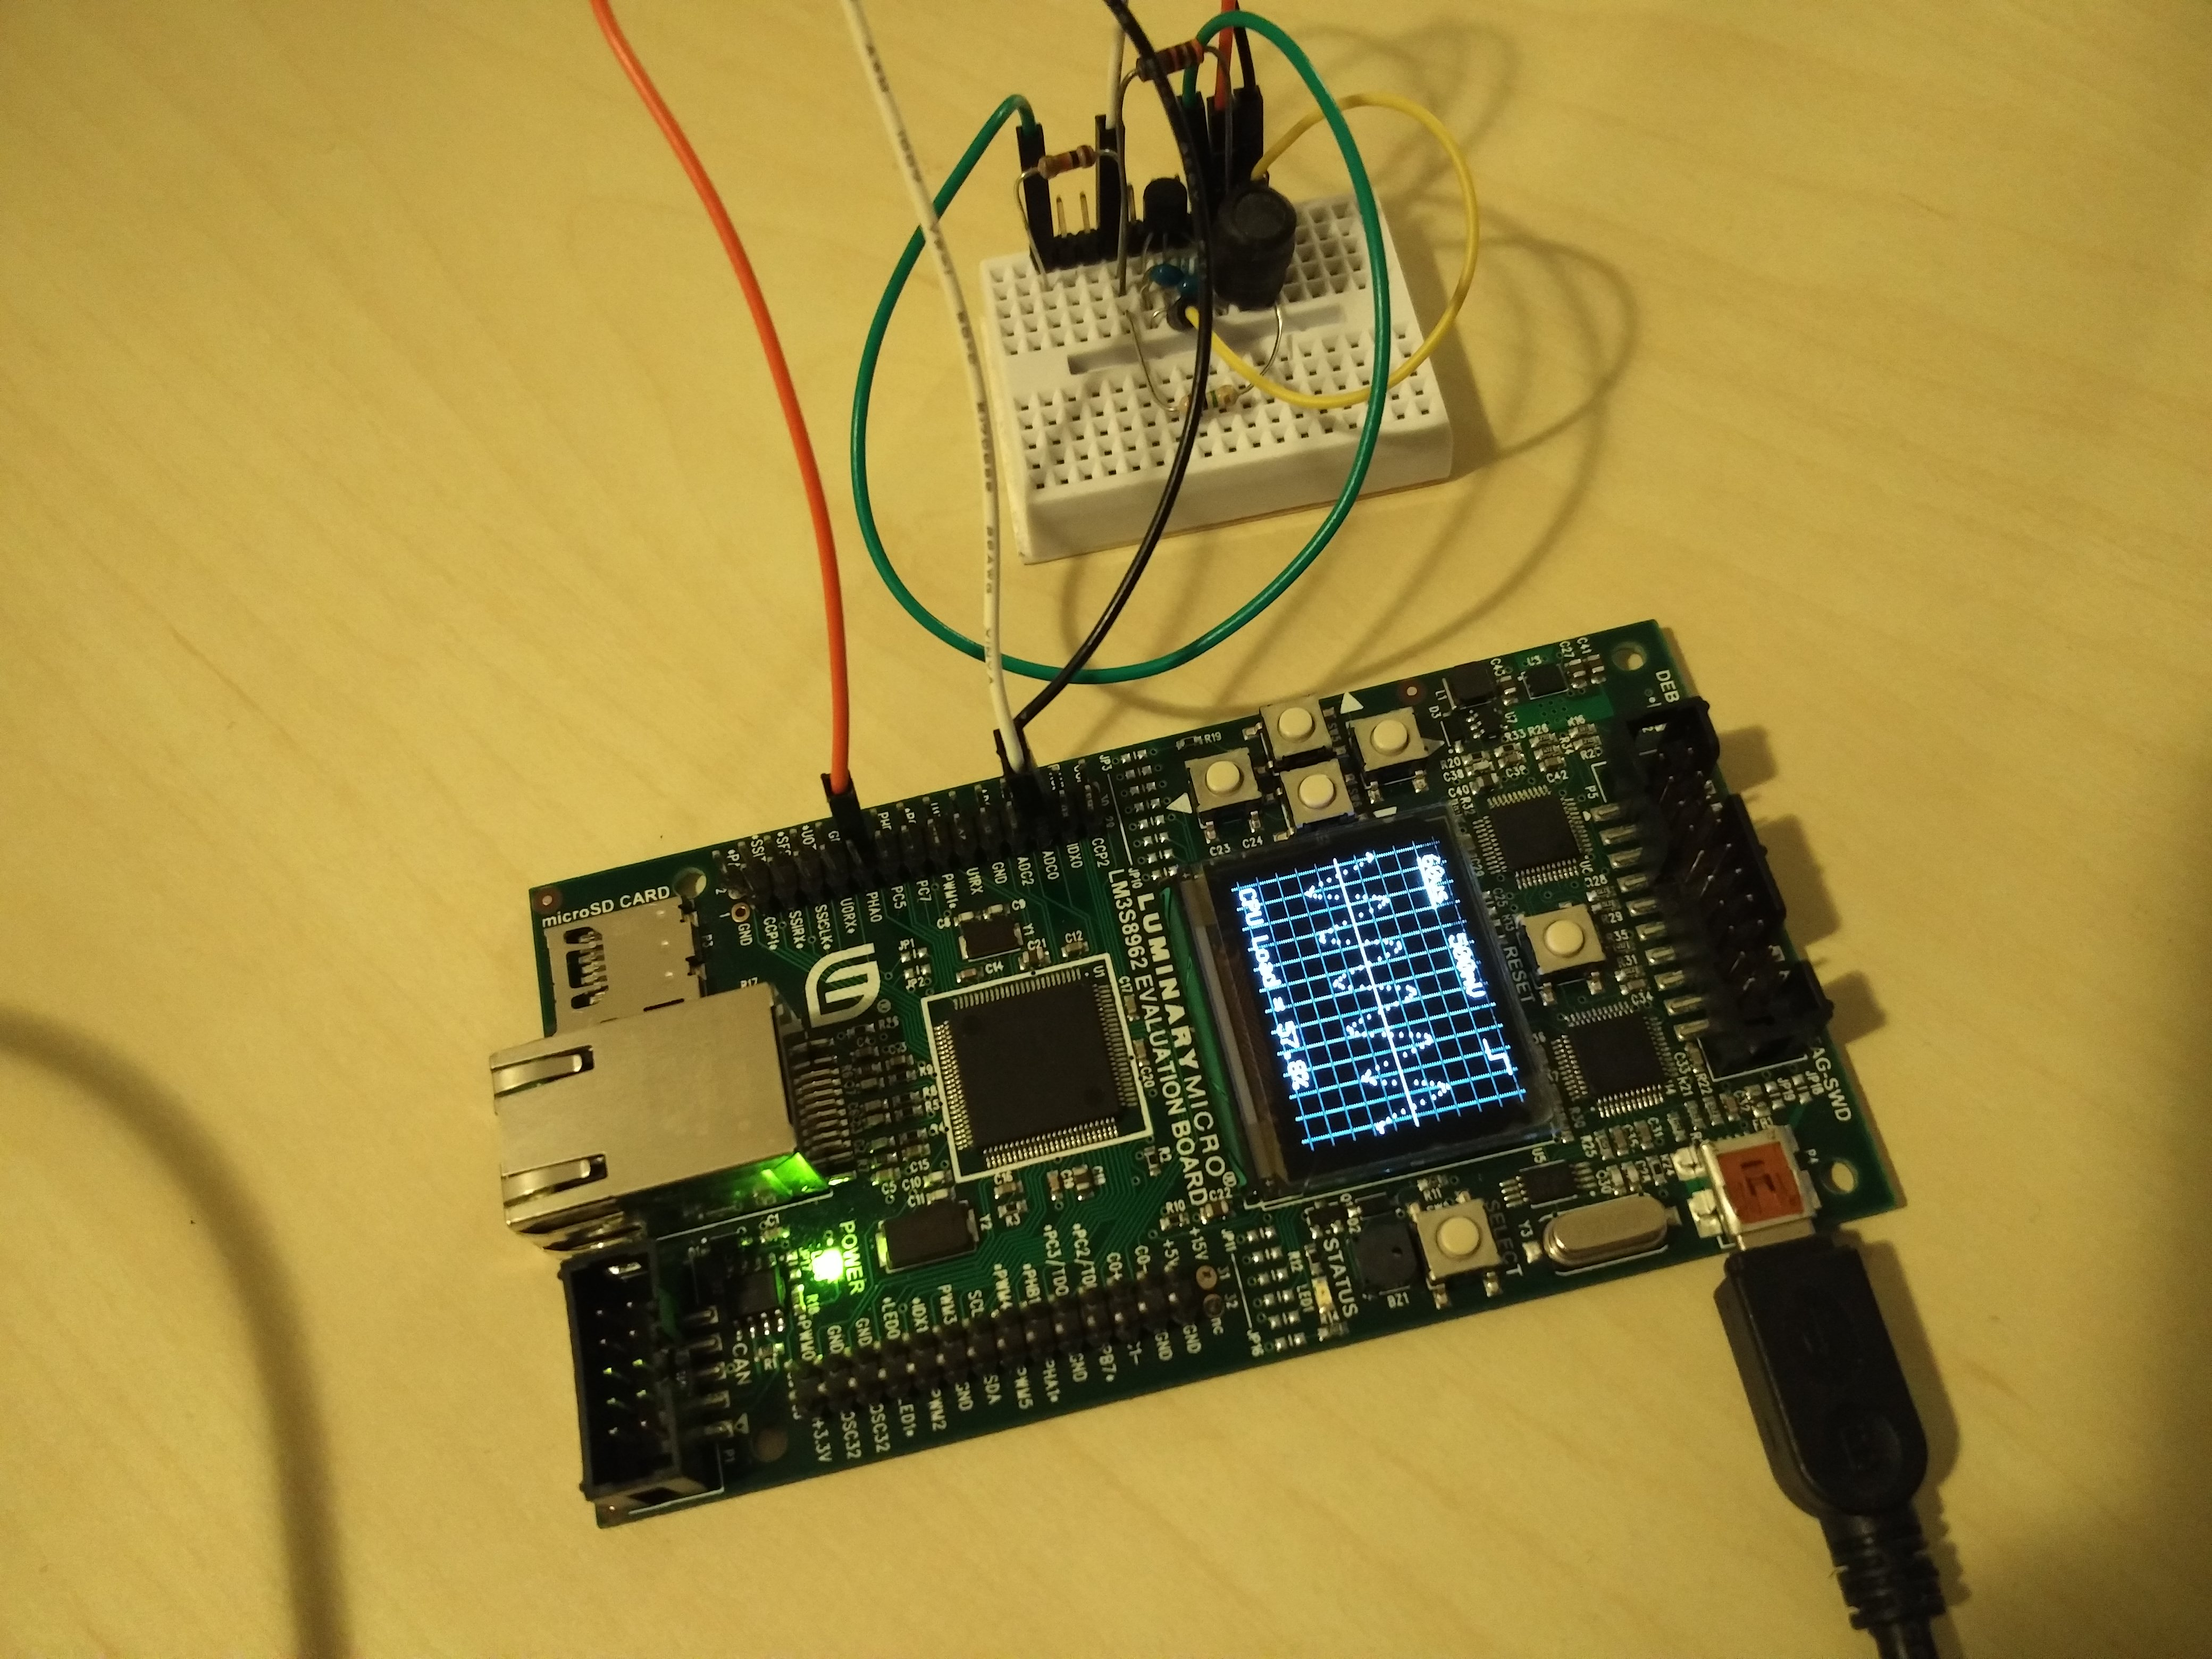
\includegraphics[width=\linewidth]{assets/overview.jpg}
  \caption{Overview of the circuit}
  \label{fig:overview}
\end{figure}

\section{Discussion and Results}
In this part we will discuss the methodologies used during the projects, along with their results.
\subsection{Building the circuit}

\begin{figure}[h]
  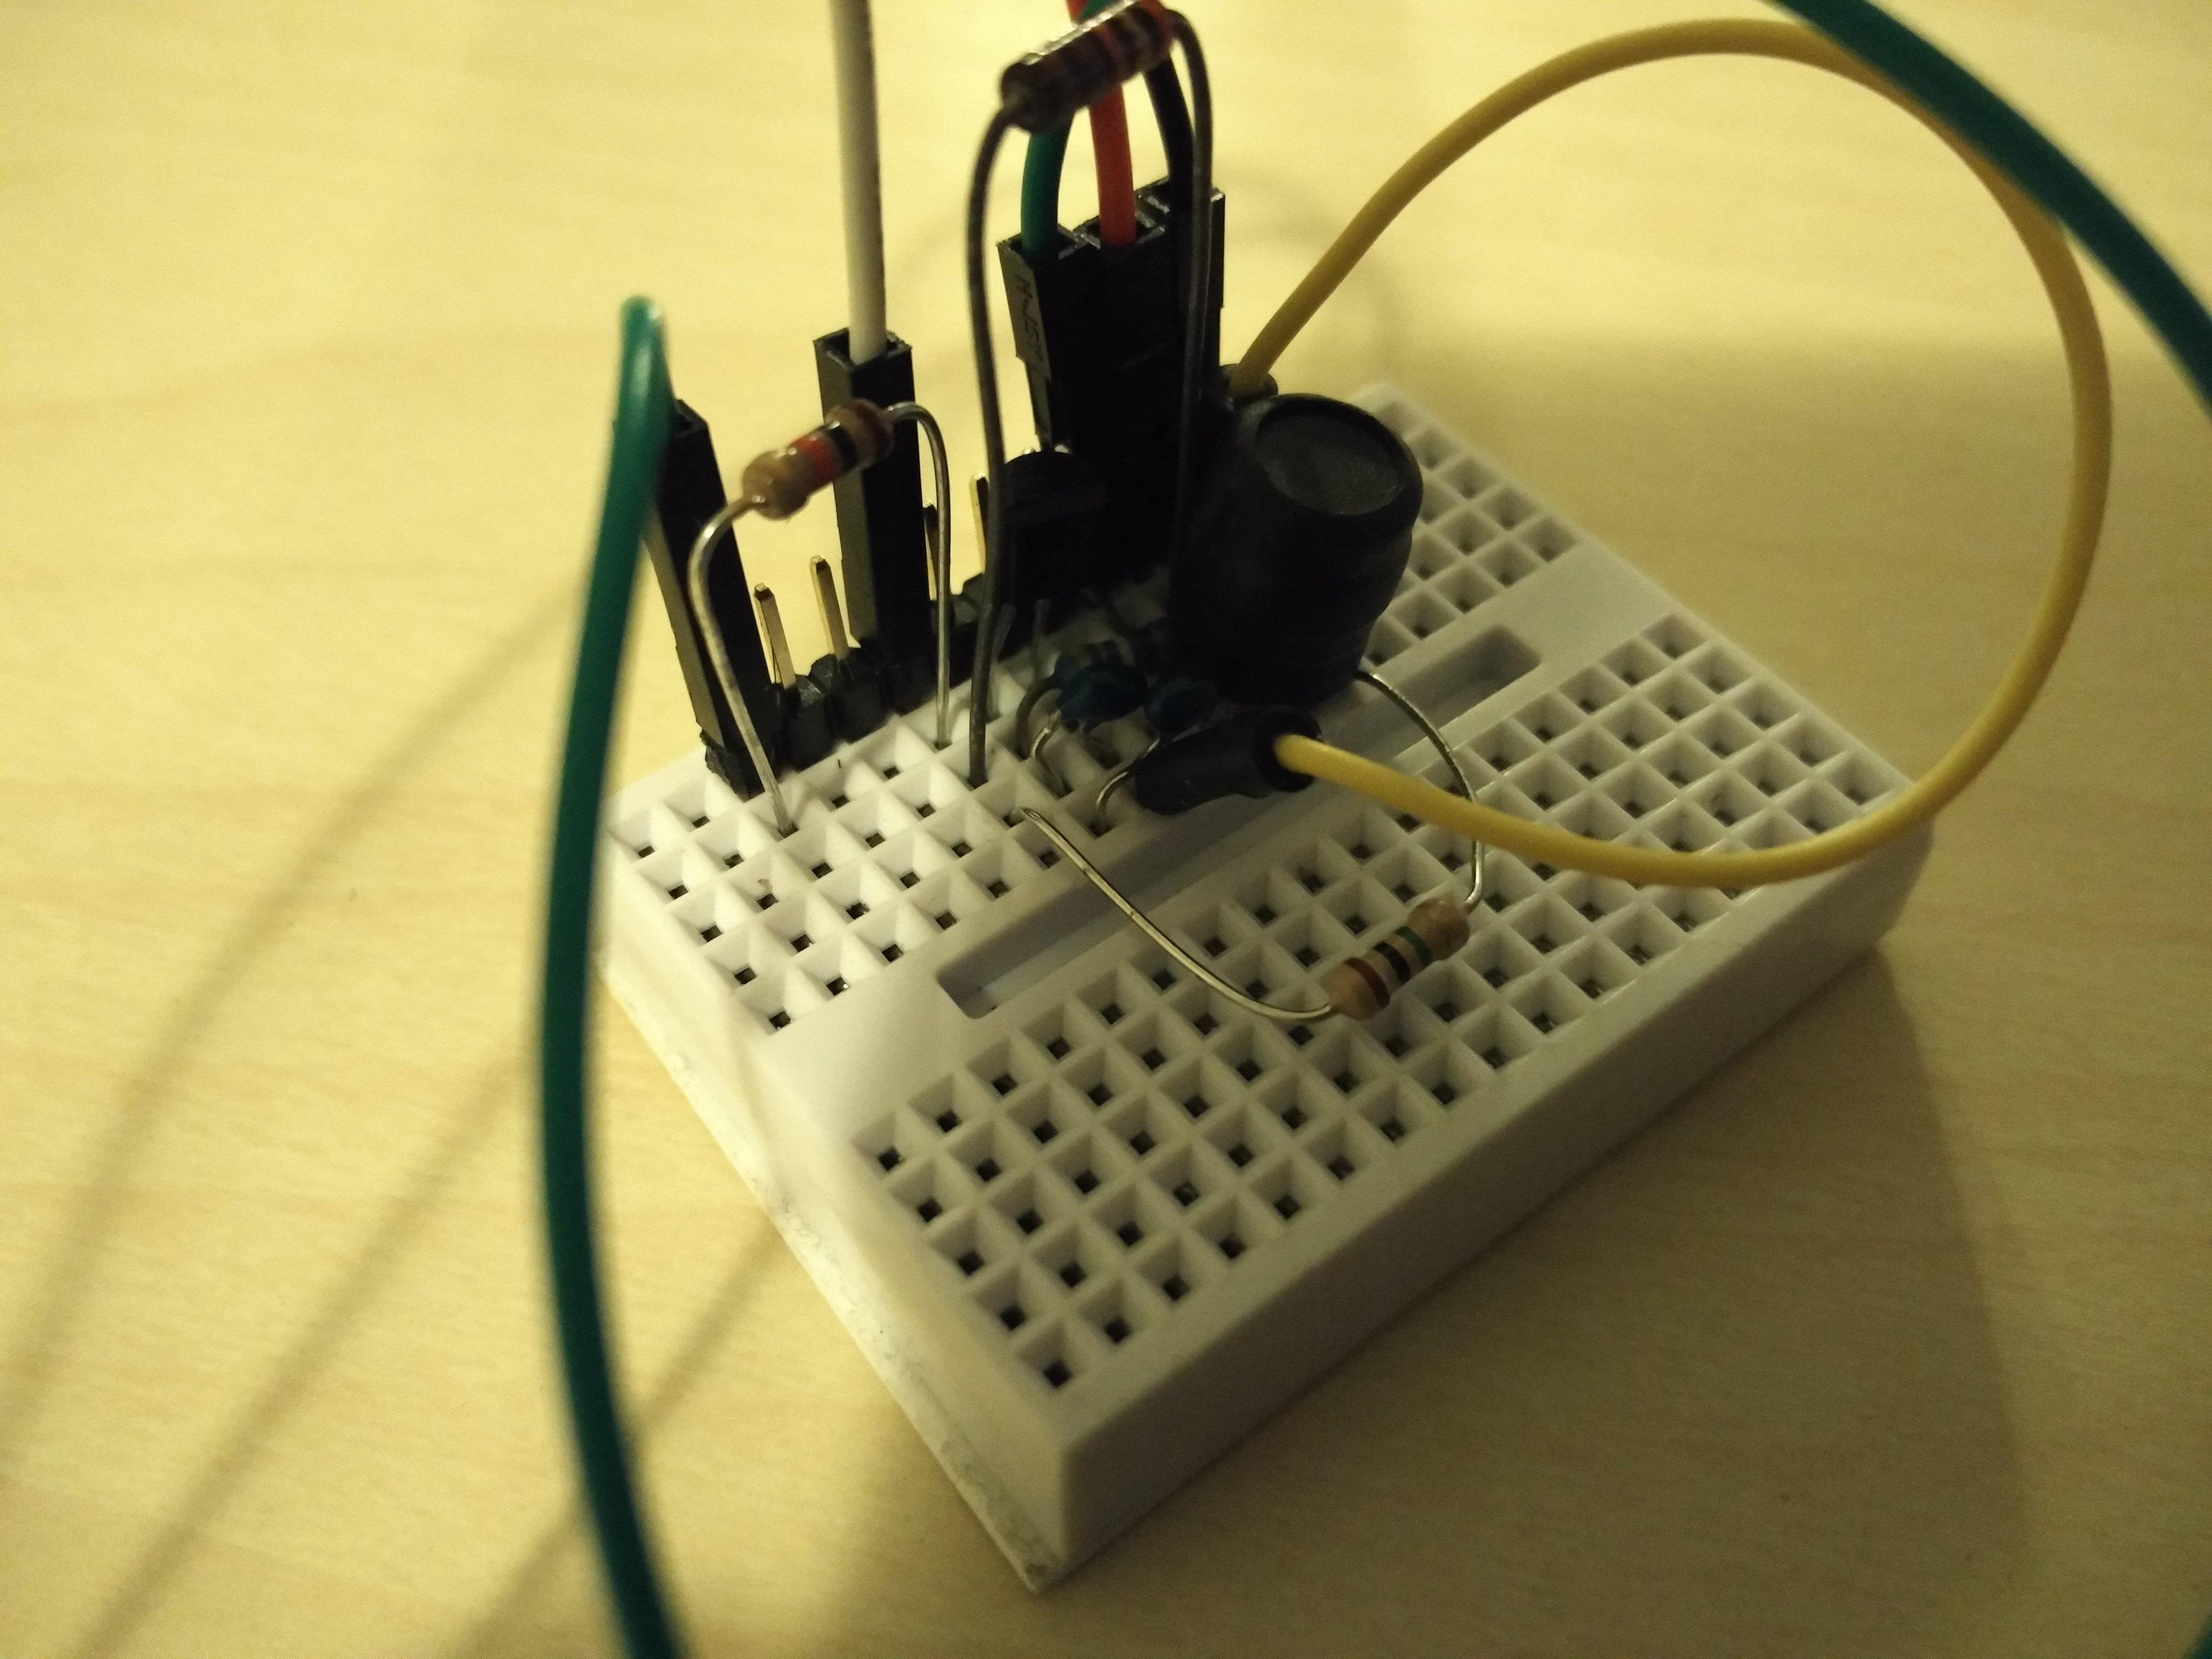
\includegraphics[width=\linewidth]{assets/circuit.jpg}
  \caption{The Colpitts oscillator}
  \label{fig:circuit}
\end{figure}

We started off by building a Colpitts oscillator from the schematic shown in our lab requirement. The resulting circuit can be seen in Figure 2. The circuit generates a (near) sine wave signal of approximate 7.1kHz, with an amplitude of approximately 0.3V, which we were able to verify using a bench scope. The signal output is then connected to a voltage divider, which maps the voltage range from -3V - 3V to 0 - 3V.

\subsection{Initializing the program}

To start the program, we have to initialize different peripherals needed for the labs. Those are: system clock, display, timers (0 through 2), buttons, and ADC. We will be looking at the code for initializing the ADC below.

\subsubsection{Initializing ADC}
Using the functions provided in the lab requirement, we filled out the parameters using macros, and the Stellaris Peripheral Driver Library User's Guide.
\lstinputlisting[firstline=504, lastline=516]{assets/main.c}

\subsection{Using interrupts}
In this subsection, we explore different roles the ISR take to make the program works.

\subsubsection{Timer0}
Timer0 is used mainly to send a pulse to blink the on-board LED, to make sure the program is running. This is mainly used for debugging/decorating purposes, and should not interfere with other main functions
\subsubsection{Timer1}
Timer1 is used to calculate the CPU load by calling \begin{verbatim} cpu_load_count() \end{verbatim} every time it is called, to update the CPU load.
\subsubsection{Timer2}
Timer2 is used to scan the button inputs, debounce them, and put them in an array to process later. Each button press in the array is identified by a different character.

\subsubsection{ADC}
The ADC0 is used for this lab experiment. During the call, it checks for FIFO overflow, increment error count if that happens, and store readings to the g\_psADCBuffer.

\subsection{Drawing screen elements}

The process of screen rendering is handled by four different functions: drawGrid, drawOverlay, drawTrigger and drawSignal. The screen is then rendered through screenDraw(), and wiped with screenClean()

\subsubsection{drawGrid}
drawGrid loops through the number of horizontal and vertical bars, and draw a line at the corresponding position.

\subsubsection{drawOverlay}
drawOverlay handles a number of different on-screen elements: time scale, voltage scale, cpu load, and trigger direction. drawOverlay also employs two helper functions, strCenter() and strWidth() to help placing and centering the text.

\lstinputlisting[firstline=647, lastline=658]{assets/main.c}
\lstinputlisting[firstline=666, lastline=676]{assets/main.c}

\subsubsection{drawTrigger}
drawTrigger simply draws a horizontal line in the middle of the screen, due to the fact that our trigger is a constant for the purpose of this lab.

\subsubsection{drawSignal}
drawSignal turned out to be more complicated than the other drawing functions, since it takes in the inputBuffer, performs a trigger search, and generates the waveform based on found values.

We start off by declaring the pixelRange, the range to display the final pixel outputs; and the pixelWidth, with is calculated by dividing the current timeScale position by the gridWidth. This ensures that the pixels are scaled to different time scales.

First we have to disable the IRQs to avoid any time-share data problems.
\lstinputlisting[firstline=314, lastline=314]{assets/main.c}

Our trigger search implementation was encapsulated in an if statement, which checks for any buffer values that pass the trigger requirements: within a range of $\pm 25$ of adcZeroValue (which would be our offset), and check for rising, or falling values by comparing it to the buffer 5 indexes behind and 5 indexes ahead.

\lstinputlisting[firstline=317, lastline=320]{assets/main.c}

If the index currently looping through was found to satisfy all requirements above, we then loop through the pixelBuffer (which is our display array), and fill it with appropriate pixels, which are calculated using pixelWidth.

\lstinputlisting[firstline=322, lastline=346]{assets/main.c}

Lastly, we enable the IRQs, and draw the pixels to the RAM, scaled appropriately to the voltage.

\lstinputlisting[firstline=349, lastline=357]{assets/main.c}

\subsubsection{Scaling}
Since the output waveform has to scale to different timeScale and voltageScale, one sample could not be interpreted as one pixel. For this, we implemented two arrays: timeNScales, and voltageNScales, which contain the values of the scale, and by using these, the pixel value can be extrapolated (e.g. pixelWidth variable in the drawSignal function). This method results in a continuous line of the signal, which makes it much clearer.

Figures 3 shows how different timeScales affect the same waveform.
\begin{figure}[!h]
\minipage{0.32\textwidth}
  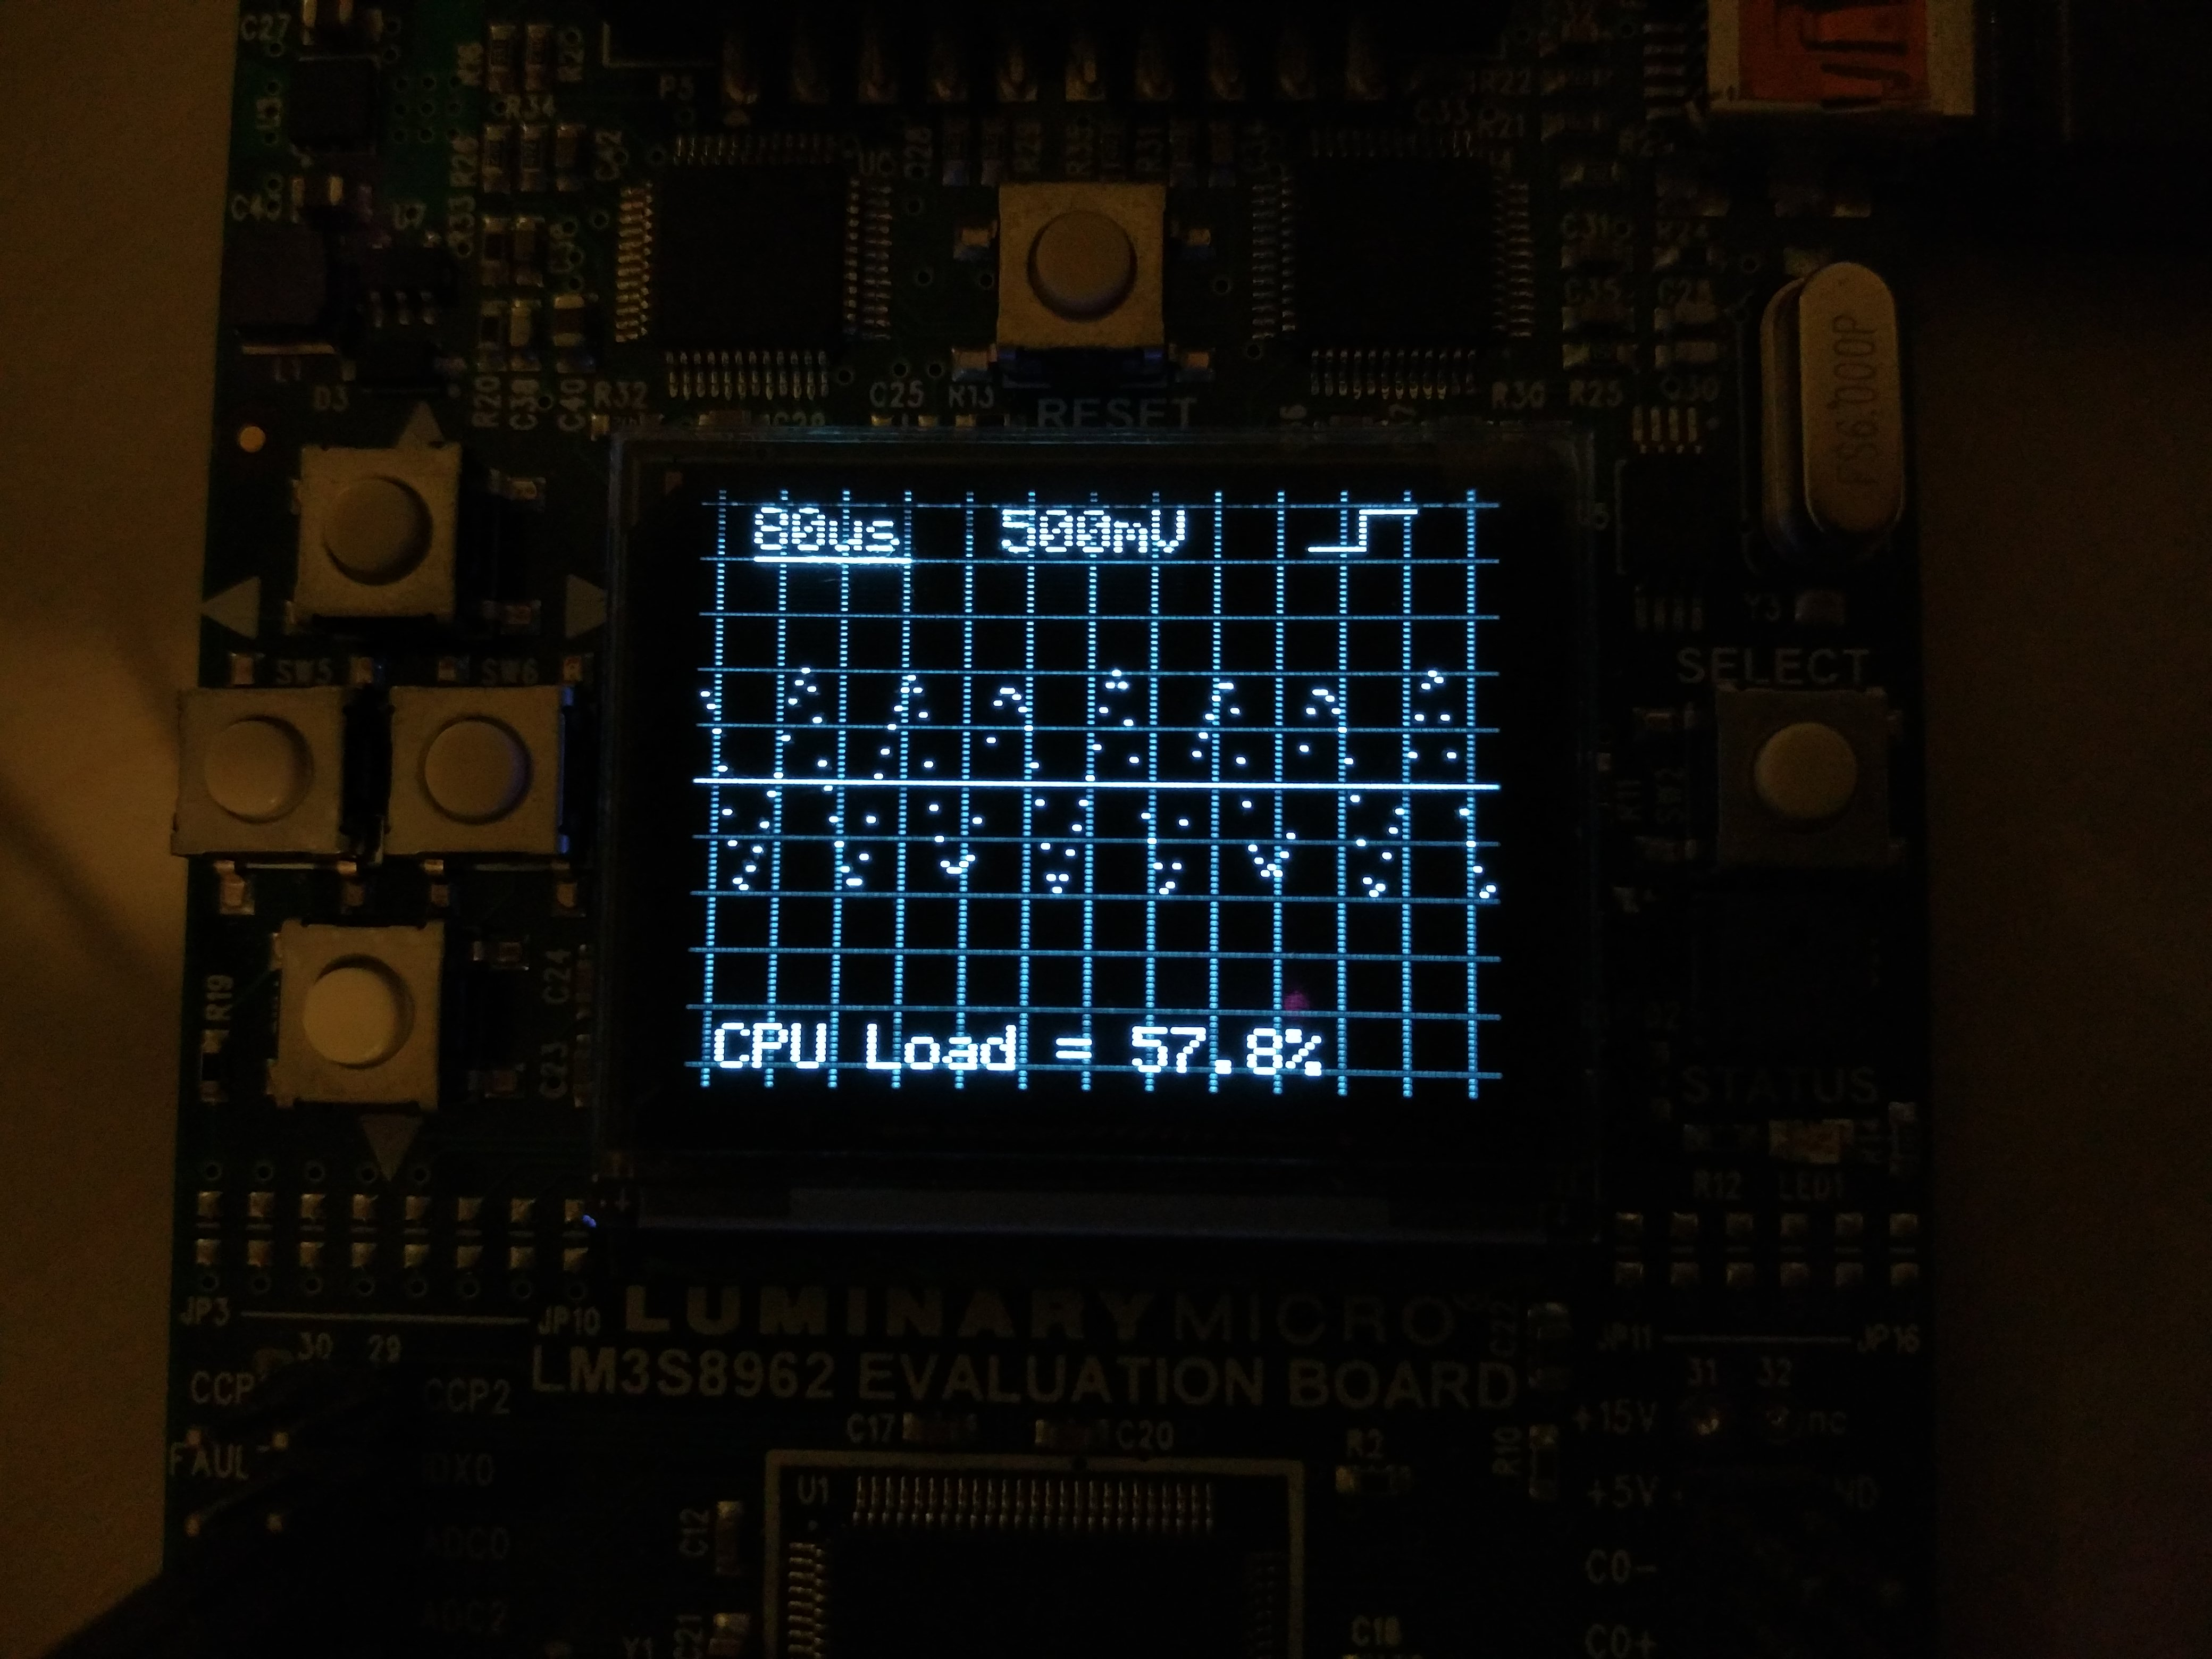
\includegraphics[width=\linewidth]{assets/wave_2.jpg}
  \caption{Timescale at 80us}\label{fig:awesome_image1}
\endminipage\hfill
\minipage{0.32\textwidth}
  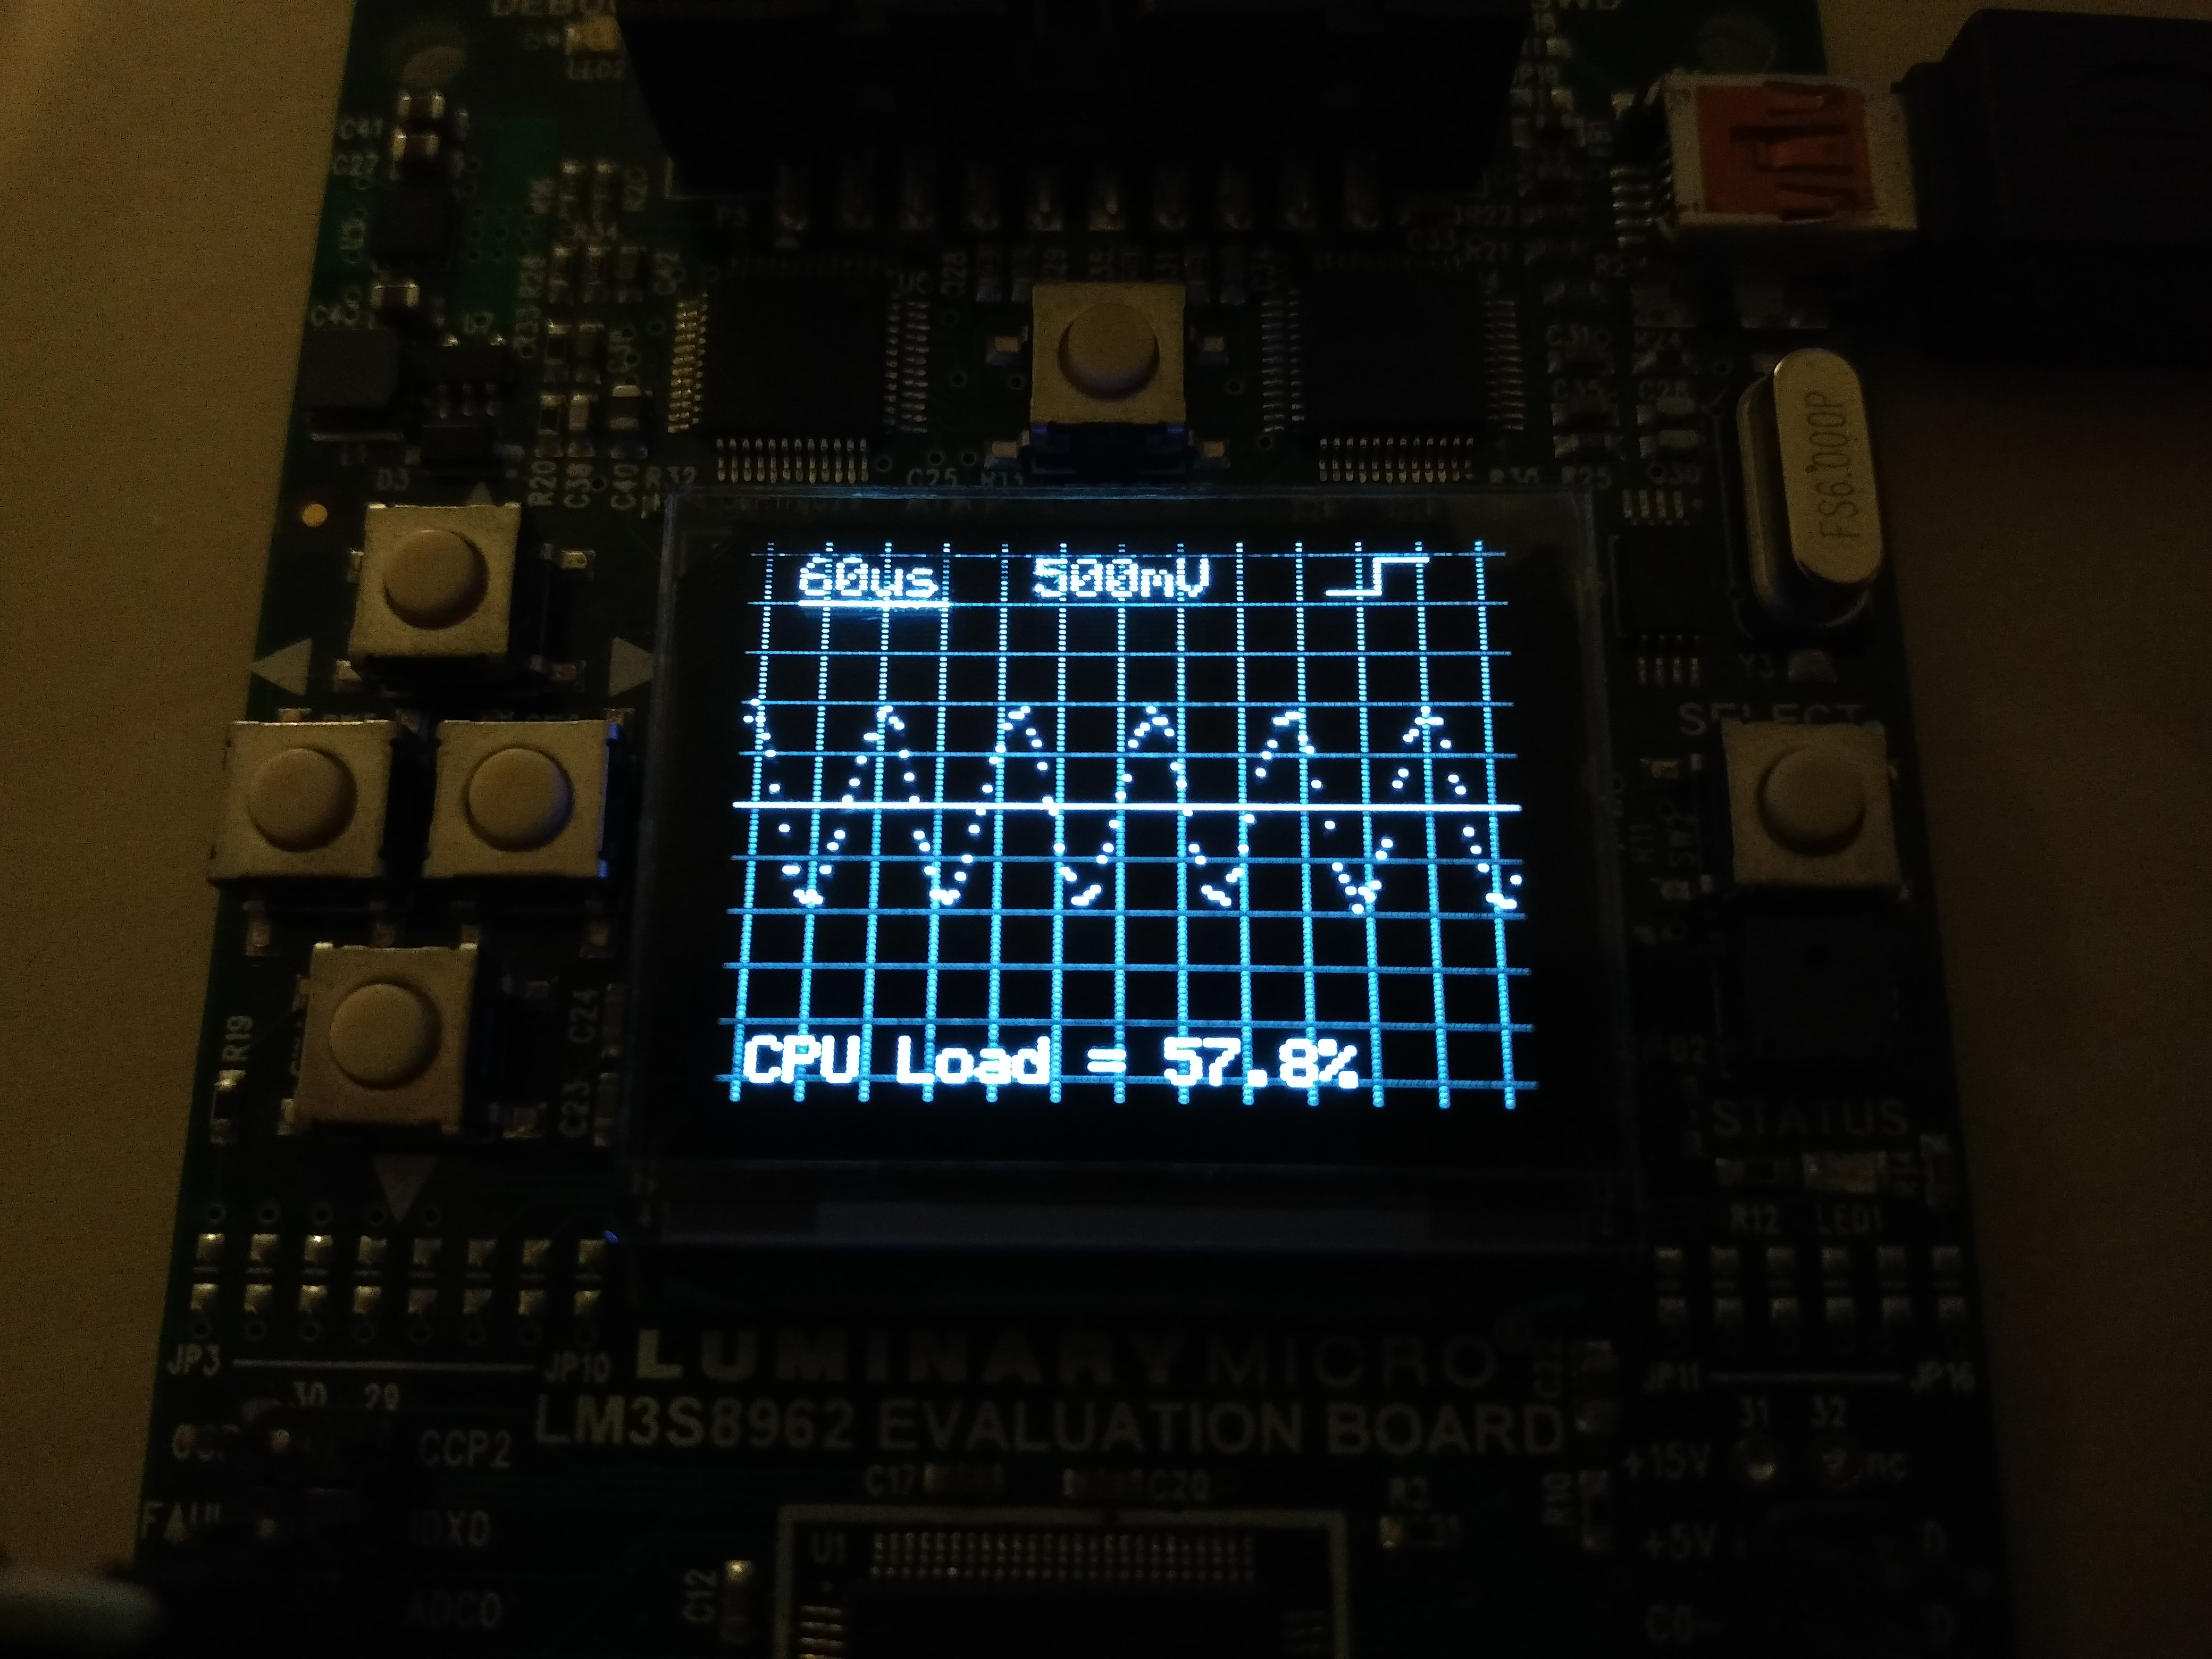
\includegraphics[width=\linewidth]{assets/wave_1.jpg}
  \caption{Timescale at 60us}\label{fig:awesome_image2}
\endminipage\hfill
\minipage{0.32\textwidth}%
  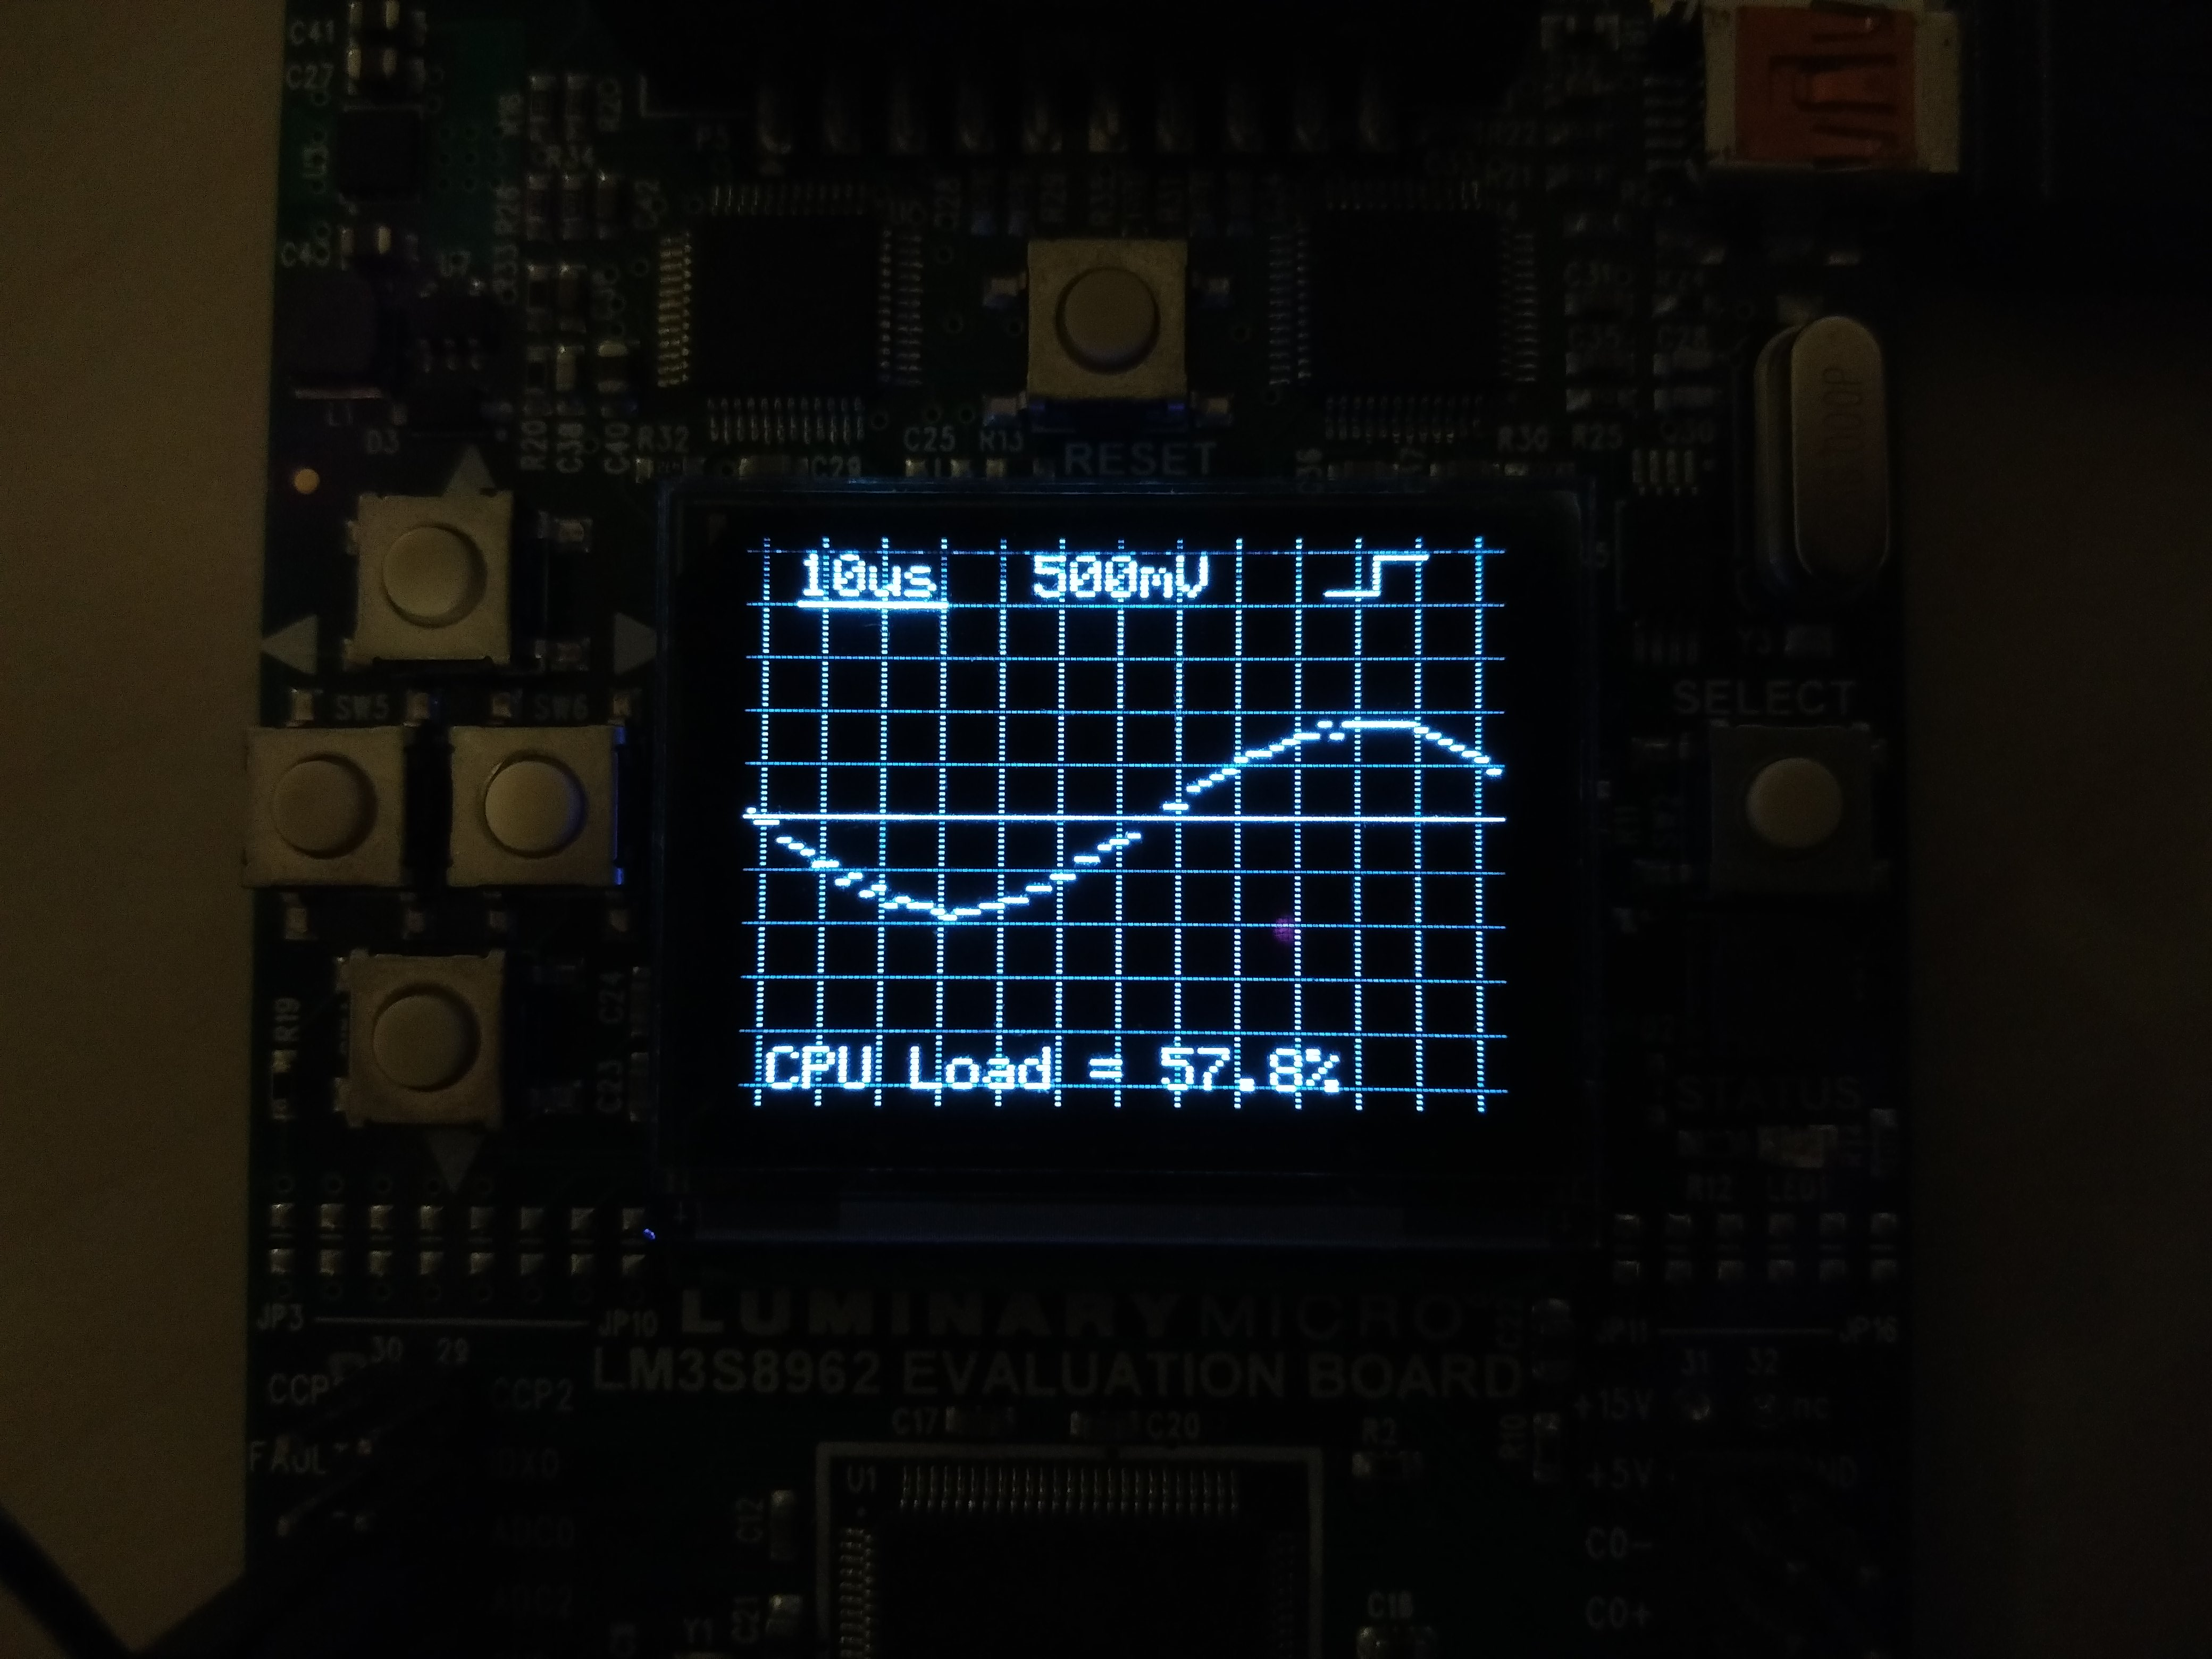
\includegraphics[width=\linewidth]{assets/wave_3.jpg}
  \caption{Timescale at 10us}\label{fig:awesome_image3}
\endminipage
\end{figure}

% \blindtext

\subsection{Handling button inputs}
Lastly, we go over how we process the button inputs while maintaining real-time functionality.

As we went through in the first section, we used Timer2 to scan the button inputs, and put them in an array. The processButtons() function, which is called in the main() function, go through the array, process them, and update the user interface accordingly based on the buttonArrayIndex.

\lstinputlisting[firstline=155, lastline=207]{assets/main.c}

\section{Conclusion}

In this lab, we got the chance to explore the basics of interrupt driven software architecture and programmed a TI Microcontroller as an oscilloscope. 

We have built a simple Colpitts oscillator and generated sine waves to measure. We saw that this circuit is not very reliable, as the components (especially the inductor) needed very good contact with the breadboard at all times. Most of the time, it worked fine to generate a 3V +/- 0.3V sine curve, which we sampled 500.000 times a second using the analog to digital (ADC) converter on chip. While this was a thight timing requirement (leaving 2 μs per sample), Cortex-M3 was up to the challenge, leaving us plenty of flops to implement other complex features as well. We have built a circullar buffer to handle samples, transfer a portion to a local buffer, map it to screen send it to the display hardware. 

We have designed a responsive graphical user interface (GUI) for the display features. Overall, our oscilloscope worked very reliably, and efficient too! With only ~58\% CPU utilization, we are proud of our code performance.

\end{document}